
\documentclass{article}

\usepackage[]{todonotes}
\usepackage[outdir=./]{epstopdf}
\usepackage[ruled]{algorithm2e}
\usepackage{amsmath}

\title{Parallel Standard Particle Swarm Optimization}
\author{Gian M. Fritsche}
\date{\today}

\begin{document}
    \maketitle

    \section{Introduction}

    The Particle Swarm Optimization~\cite{PSO95} is a meta-heuristic based on the behavior of bird flocks. Every iteration, each particle moves in the search space based on three components:

    \begin{itemize}
        \item {\em Social:} This component contributes for the exploitation of the algorithm.
        It guides the search towards the best solutions found by the swarm.
        \item {\em Individual:} The individual component guides the particle to the best region that the particle has found.
        \item {\em Inertia:} The inertia component increase the exploration of the algorithm. It is responsible for keeping the particle moving towards a previous direction and avoid abrupt changes of direction.
    \end{itemize}

    The position of one particle is a set of variable values, {\em i.e.} a solution for an optimization problem. Then, the algorithms evaluate the solution, and a fitness value is associated. Based on the fitness value the Social and Individual components are updated.
    Moreover, these components are used to compute the next position of the particle (another solution for the problem).

    Since its first publication, the PSO had proposed several adaptations and improvements.
    In 2006 it was created the first version of a Standard Particle Swarm Optimization~\cite{SPSO}. The SPSO was not proposed to be the best PSO available, but establish a common benchmark as a baseline to assess the PSO variants in the literature.

    \subsection {Standard Particle Swarm optimization}

    Since its first publication (2006), there is three versions of SPSO: 2006, 2007 and 2011.
    In the latest version the description is given as follow (and showed in Algorithm~\ref{alg:spso2011}):
    The first population (set of solutions) is initialized randomly in the search space. Then, the algorithms initialize the velocity also randomly. The suggested population size is $40$. The neighborhood topology used to update the social component is the Adaptive Random Topology (ART).
    In the ART each particle informs its current fitness to $K$ neighbors. If the fitness is better than the previous social best information of the neighbor the social best (fitness and position) is updated. A direct graph represents the neighborhood, where each particle informs its quality to (at most) $K$ neighbors. The graph is generated randomly initially and every time that the best global fitness is not improved.

    In the previous versions of PSO, the velocity was updated dimension by dimension.
    However, in SPSO2011 the velocity is updated in a geometrical way,  that does not depend on the system of coordinates.

    \begin{algorithm}[!htb]
        \KwResult{The best solution and its fitness}
        
        create adaptive random neighbourhood\;

        \ForEach{particle $ i \in swarm$}{
            initialize particles' position ($\vec{X_i}$) and velocity ($\vec{V_i}$)\;
            evaluate particle ($f(\vec{X_i})$)\;
            initialize personal best ($\vec{P_i}$) and neighbour best ($\vec{G_i}$)\;
            update global best fitness ($best\_fitness=\min(f(\vec{X_i}), best\_fitness)$)\;
        }
        number of iterations ($T$) = 1\;
        \While{$T < MAX\_IT$  }{
            $previous\_best\_fitness = best\_fitness$\;
            \ForEach{particle $ i \in swarm$}{
                update particle's velocity ($\vec{V_i}$)\;
                update particle's position ($\vec{X_i}$)\;
                evaluate particle ($f(\vec{X_i})$)\;
                \If{ $f(\vec{X_i}) < f(\vec{P_i})$ }{
                    $\vec{P_i} = \vec{X_i}$\;
                }
                update neighbour best ($\vec{G_i}$)\;
                update global best fitness ($best\_fitness=\min(f(\vec{X_i}), best\_fitness)$)\;
            }
            \If{$previous\_best\_fitness \le best\_fitness$}{
                create adaptive random neighbourhood\;
            }

            $T=T+1$
        }
        \ForEach{particle $ i \in swarm$}{
            \If{$f(\vec{X_i}) == best\_fitness$}{
                $best\_solution = \vec{X_i}$\; 
            }
        }
        
        \caption{Standard Particle Swarm Optimization 2011}
        \label{alg:spso2011}
    \end{algorithm}

    \section{Parallel SPSO-2011}

    \subsection{Related works}

    In the literature, it is possible to find different proposals of Parallel PSOs.
    One of the most recent is the GPU-based Asynchronous Particle Swarm Optimization~\cite{GPUPSO}.
    That implements a simple ring topology.
    In~\cite{ReviewGPUPSO}, it is presented a review of Particle Swarm Optimization on GPU.
    The paper presents 28 references of PSO on GPU including multi-objective versions and variations of PSO from 2009 to 2014.
    One of the papers from the review implements the Standard Particle Swarm Optimization 2007 using GPU~\cite{GPUSPSO2007}. The GPU version was 11 times faster than the CPU, mainly with a large population and high dimensional problems.

    \subsection{Proposal}

    In this work, we use the SPSO2011, which uses the Adaptive Random Neighborhood topology.  
    During the literature review, it was not found any other implementation of the SPSO2011 using GPU.
    The parallel implementation associates each particle with one thread (Algorithm~\ref{alg:pspso2011}).
    In this way, all \texttt{{\bf foreach} particle $ i \in swarm$ } were removed and executed in parallel based on the thread id inside the block ($threadIdx.x$ or $tid$).
    In the create adaptive random neighborhood method each particle selects up to $K$ neighbors. Then the particle updates its position and velocity; the position is evaluated using the fitness function, and the personal best is updated.
    Then, to update the neighbor best information, the particle search on the adjacency matrix of the neighborhood for all its neighbors and compares to itself.
    The best global fitness is computed using atomic operations. The $atomicMin(a, b)$ was implemented based on the CUDA $atomicCAS$, which realizes a compare and swap operation.
    Before entering the main loop, the implementation applies a thread synchronization.

    The first particle copies the best fitness for later comparison.
    Inside the main loop, the particle (thread) updates its velocity, position, and fitness.
    The personal best information is updated.
    Before set the neighbor best information a synchronization is necessary because the threads must compare its fitness to the updated value of its neighbors.
    Then, the neighbor best information is updated. Also, the best fitness is updated using the $atomicMin$ function.
    After the best fitness update, it is applied another \texttt{\_\_syncthreads()}. To wait for all threads update the best fitness before using its value.
    If the best fitness is not improved, then the new neighborhood matrix is generated.
    After $T$ iterations the solution with fitness equals to the best fitness is the output of the algorithm.

    \begin{algorithm}[!htb]
        \KwResult{The best solution and its fitness}
        
        $tid = threadIdx.x\;$

        create adaptive random neighbourhood\;
        \_\_syncthreads()\;

        initialize particles' position ($\vec{X_{tid}}$) and velocity ($\vec{V_{tid}}$)\;
        evaluate particle ($f(\vec{X_{tid}})$)\;
        initialize personal best ($\vec{P_{tid}}$) and neighbour best ($\vec{G_{tid}}$)\;
        \tcc{the update global best uses atomicMin operation}
        update global best fitness ($best\_fitness=\min(f(\vec{X_{tid}}), best\_fitness)$)\;
        \_\_syncthreads()\;
        number of iterations ($T$) = 1\;
        \While{$T < MAX\_IT$  }{
            \If{$tid == 0$}{
                $previous\_best\_fitness = best\_fitness$\;
            }
            
            update particle's velocity ($\vec{V_{tid}}$)\;
            update particle's position ($\vec{X_{tid}}$)\;
            evaluate particle ($f(\vec{X_{tid}})$)\;
            \If{ $f(\vec{X_{tid}}) < f(\vec{P_{tid}})$ }{
                $\vec{P_{tid}} = \vec{X_{tid}}$\;
            }
            \_\_syncthreads()\;
            update neighbour best ($\vec{G_{tid}}$)\;
            \tcc{the update global best uses atomicMin operation}
            update global best fitness ($best\_fitness=\min(f(\vec{X_{tid}}), best\_fitness)$)\;
            \_\_syncthreads()\;
            
            \If{$previous\_best\_fitness \le best\_fitness$}{
                create adaptive random neighbourhood\;
            }

            $T=T+1$
        }
        
        \If{$f(\vec{X_{tid}}) == best\_fitness$}{
            $best\_solution = \vec{X_{tid}}$\; 
        }
        
        \caption{Parallel Standard Particle Swarm Optimization 2011}
        \label{alg:pspso2011}
    \end{algorithm}

    In the first implemented version it was not used shared memory, but in a second implementation it was used and the execution time was improved.
    Another item important to highlight is the two \texttt{\_\_syncthreads()} inside the loop.
    The use of \texttt{\_\_syncthreads()} generally slow down the execution of a CUDA program.
    % However, in this implementation we did not have this problem due to the block size equals to warp size.
    % Since the threads in the same warp execute in true (hardware) parallelism, there is no situation where threads need to sync with others on the same block.

    The first experiments were executed using only one block. However, the experiments run the SPSO several times; those executions can be run in parallel, using different and independent blocks. In the experiments using only one block the CPU implementation had a better execution time. However, when using multi executions at once, the GPU implementation achieved a better execution time.
    Those first experimets were executed using a simple function called Sphere.
    Then it was evaluated the scalability of the implementations increasing the population size. The population size defines the number of threads per block. For those experiments it was used the Schaffer function.
    The next section details the experiments and results.

    \section{Experiments and Results}

    The first experiment was used to validate the equivalence regarding the quality of the GPU and CPU implementation. Both implementations showed similar convergence along the execution.

    For this first experiments it was used $T=3125$ iterations, $32$ particles, $D=10$ decision variables, $K=3$, and the Sphere function for fitness evaluation (this function is presented in Figure~\ref{fig:sphere}).  We executed $51$ independent runs. Those parameters were based on~\cite{SPSOCEC}. Moreover, the Sphere function is a simple optimization function present on the COCO (Comparing Continuous Optimisers) benchmark~\footnote{http://coco.gforge.inria.fr/}. The Sphere function is a minimization problem: 

    \begin{equation}
        f(x_1 \cdots x_n) = \sum_{i=1}^n x_i^2
    \end{equation}

    \begin{equation}
            -100.0 \leq x_i \leq 100.0
    \end{equation}

    \begin{equation}
       \text{minimum at }f(0, \cdots, 0) = 0
    \end{equation}

     \begin{figure}[!htb]
        \centering
        \includegraphics[width=.7\textwidth]{../img/sphere.png}
        \caption{Sphere --- Two dimensional view}
        \label{fig:sphere}
    \end{figure}


    The Table~\ref{tbl:gpuinfo} presents the information about the used GPU.
    Besides, the Table~\ref{tbl:cpuinfo} presents the CPU information.

    \begin{table}[!htb]
        \centering
        \caption{GPU information}
        \label{tbl:gpuinfo}
        \begin{tabular}{|l|l|}
            \hline
            \multicolumn{2}{|c|}{\textbf{--- General Information for device 0 ---}} \\ \hline
            \textbf{Name}                          & GeForce GTX 680                \\ \hline
            \textbf{Compute capability}            & 3.0                            \\ \hline
            \textbf{Clock rate}                    & 1058500                        \\ \hline
            \textbf{Device copy overlap}           & Enabled                        \\ \hline
            \textbf{Kernel execution timeout}      & Disabled                       \\ \hline
            \multicolumn{2}{|c|}{\textbf{--- Memory Information for device 0 ---}}  \\ \hline
            \textbf{Total global mem}              & 2095382528                     \\ \hline
            \textbf{Total constant Mem}            & 65536                          \\ \hline
            \textbf{Max mem pitch}                 & 2147483647                     \\ \hline
            \textbf{Texture Alignment}             & 512                            \\ \hline
            \multicolumn{2}{|c|}{\textbf{--- MP Information for device 0 ---}}      \\ \hline
            \textbf{Multiprocessor count}          & 8                              \\ \hline
            \textbf{Shared mem per mp}             & 49152                          \\ \hline
            \textbf{Registers per mp}              & 65536                          \\ \hline
            \textbf{Threads in warp}               & 32                             \\ \hline
            \textbf{Max threads per block}         & 1024                           \\ \hline
            \textbf{Max thread dimensions}         & (1024, 1024, 64)               \\ \hline
            \textbf{Max grid dimensions}           & (2147483647, 65535, 65535)     \\ \hline
        \end{tabular}
    \end{table}

    \begin{table}[!htb]
        \centering
        \caption{CPU information}
        \label{tbl:cpuinfo}
        \begin{tabular}{|l|l|}
            \hline
            \textbf{vendor\_id} & GenuineIntel                             \\ \hline
            \textbf{cpu family} & 6                                        \\ \hline
            \textbf{model}      & 63                                       \\ \hline
            \textbf{model name} & Intel(R) Core(TM) i7-5930K CPU @ 3.50GHz \\ \hline
            \textbf{stepping}   & 2                                        \\ \hline
            \textbf{microcode}  & 0x36                                     \\ \hline
            \textbf{cpu MHz}    & 3599.941                                 \\ \hline
            \textbf{cache size} & 15360 KB                                 \\ \hline
        \end{tabular}
    \end{table}

    In the Figure~\ref{fig:semilogy_convergence} it is presented the average convergence of the algorithms (GPU and CPU) during the iterations. Where it is possible to observe similar behavior because they implement the same algorithm.
    As increasing the number of iteration better is the quality of the solutions. 
    That indicates that the implementations of GPU and CPU are equivalent in terms of solution quality.

    % \begin{figure}[!htb]
    %     \centering
    %     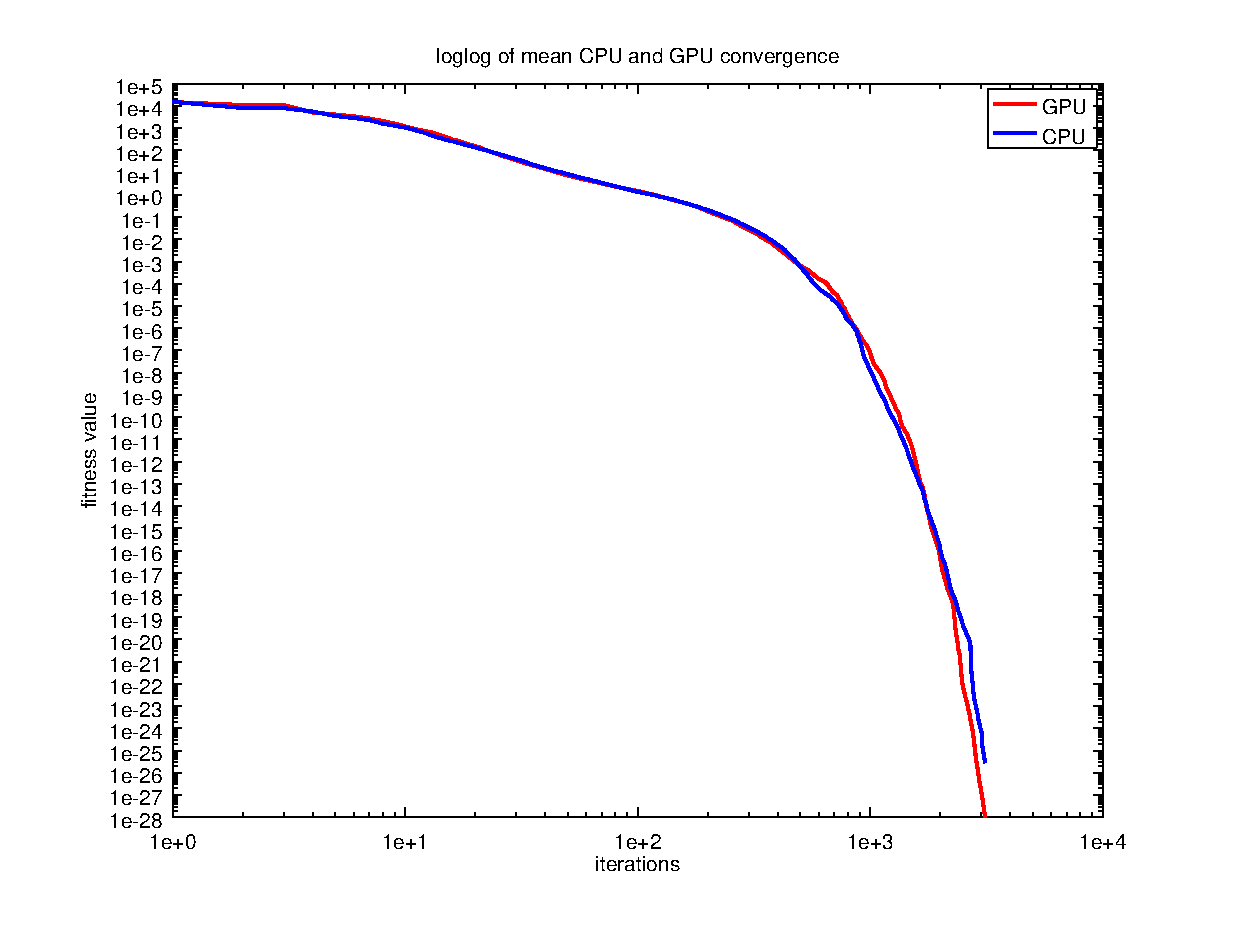
\includegraphics[width=.7\textwidth]{../img/loglog_convergence.eps}
    %     \caption{loglog of the average quality of the solutions found by the implemented algorithms during the $3125$ iterations. As much more iterations, better is the quality of the solutions. Both CPU and GPU behaves similarly, as they implement the same algorithm}
    %     % \caption{loglog of mean CPU and GPU convergence}
    %     \label{fig:loglog_convergence}
    % \end{figure}

    \begin{figure}[!htb]
        \centering
        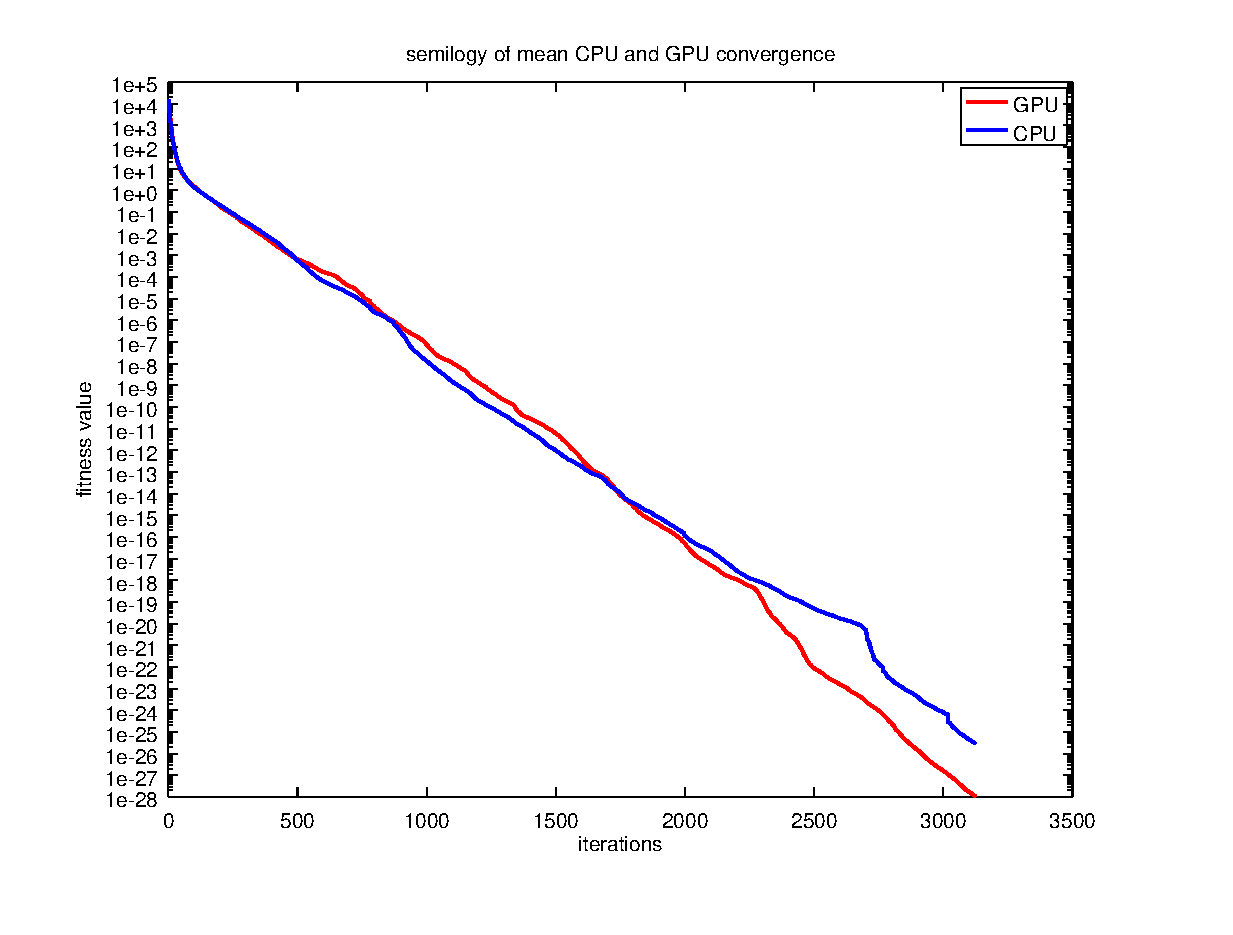
\includegraphics[width=.7\textwidth]{../img/semilogy_convergence.eps}
        \caption{semilogy of the average quality of the solutions found by the implemented algorithms during the $3125$ iterations on the Sphere problem with $10$ dimensions. As much more iterations, better is the quality of the solutions. Both CPU and GPU behaves similarly, as they implement the same algorithm. For this experiment the GPU implements $1$ block of $32$ threads and this experiment was repeated $51$ times}
        \label{fig:semilogy_convergence}
    \end{figure}

    Then, we implemented a version using shared memory also.
    The best-known fitness, the previous best, the population (or swarm), the fitness values and the adjacency matrix use shared memory.
    We compare the three versions (CPU, GPU, and GPU with shared memory). In terms of convergence the results were similar (as they should [Figure~\ref{fig:sphere10_32particles_fitness}]).
    That indicates that the GPU implementation using shared memory is equivalent to the previous GPU and CPU version in terms of quality of solutions.
    The experiments were repeated $51$ times with the GPU versions using just one block with $32$ threads. The GPU with shared memory was $1.1377$ times faster in average than GPU without using shared memory. But, the CPU implementation was the fastest: $2.87$ times faster than GPU (Figure~\ref{fig:sphere10_32particles_time}).
    Those results shows that the GPU using only one block of $32$ threads is not competitive against the CPU. As the implementation using shared memory was faster than the previous one, it is the default GPU implementation used on the next experiments.


    \begin{figure}[!htb]
        \centering
        \includegraphics[width=.7\textwidth]{../img/sphere10_32particles_fitness.eps}
        \caption{Boxplot of the quality of the output solution set generated by the algorithms (CPU, GPU and GPU using shared memory) on the Sphere problem with $10$ dimensions. All implementations behave similarly (in terms of quality of result) as they implement the same algorithm. Both GPU implementations use $1$ block of $32$ threads and this experiment was repeated $51$ times.}
        % \caption{Convergence of different implementations (single block - 51 executions)}
        \label{fig:sphere10_32particles_fitness}
    \end{figure}


    \begin{figure}[!htb]
        \centering
        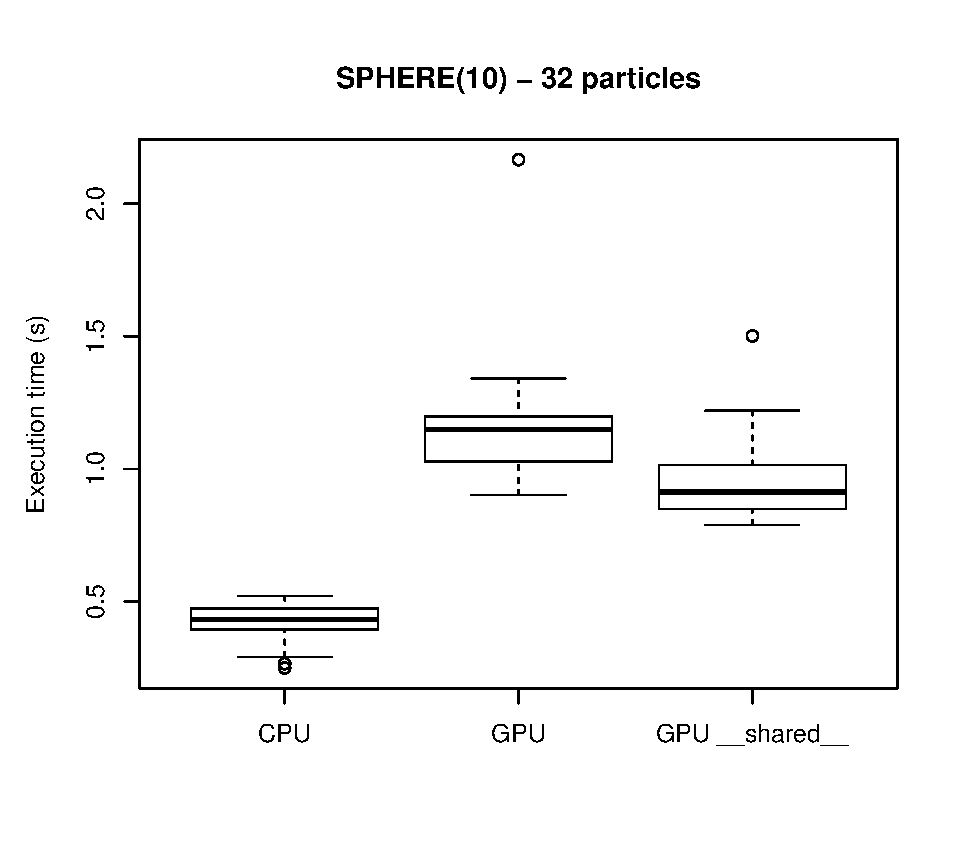
\includegraphics[width=.7\textwidth]{../img/sphere10_32particles_time.eps}
        \caption{Boxplot of the exexution time (in seconds) of the implemented algorithms (CPU, GPU and GPU using shared memory) on the Sphere problem with $10$ dimensions. Both GPU implementations use $1$ block of $32$ threads and this experiment was repeated $51$ times. In this experiment the CPU version was about $3$ times faster then GPUs, running in most cases in less than half second. The GPU versions executed generally close to one second, but the version with shared memory ran faster. (Experiments with more threads and blocks are presented further)}
        % \caption{Execution time of different implementations (single block - 51 executions)} 
        \label{fig:sphere10_32particles_time}
    \end{figure}


    \subsection{Multi-blocks experiments}

    To use the CUDA parallelism capabilities and exploit the characteristics of SPSO it was created another GPU code implementation that executes the $51$ runs in parallel using $51$ blocks. To evaluate the execution time we repeat the experiment $30$ times. For comparison it was also implemented a CPU version that compute the $51$ independent runs but iteratively.
    Again it is first evaluated if the quality of the result is equivalent between the CPU and GPU implementations.
    The fitness of the GPU (with shared memory) and CPU continued to be similar (Figure~\ref{fig:sphere10_32particles_multi_runs_fitness}) but the execution time of the GPU was faster than CPU (Figure~\ref{fig:sphere10_32particles_multi_runs_time}).
    Using $51$ blocks to execute the $51$ independent runs of the algorithm the GPU implementation was $12$ times faster then CPU. The execution of the GPU code took $0.346$ seconds in average. While the CPU code took $12.849$ seconds in average.


    \begin{figure}[!htb]
        \centering
        \includegraphics[width=.7\textwidth]{../img/sphere10_32particles_multi_runs_fitness.eps}
        \caption{Boxplot of the quality of the solutions generated by CPU and GPU (with shared memory) versions on the Sphere problem with $10$ dimensions. In this experiment the GPU uses $51$ blocks of $32$ threads and the experiment was repeated $30$ times. The implementations behave similarly (in terms of quality) as they implement the same algorithm.}
        \label{fig:sphere10_32particles_multi_runs_fitness}
    \end{figure}


    \begin{figure}[!htb]
        \centering
        \includegraphics[width=.7\textwidth]{../img/sphere10_32particles_multi_runs_time.eps}
        \caption{Boxplot of the execution time (in seconds) of CPU and GPU (with shared memory) on the Sphere problem with $10$ dimensions. In this experiment the GPU uses $51$ blocks of $32$ threads and the experiment was repeated $30$ times. The GPU was $12$ times faster than CPU.}
        % \caption{Execution time of different implementations (GPU 51-blocks, 30 repetitions)}
        \label{fig:sphere10_32particles_multi_runs_time}
    \end{figure}


    \subsection{Scalability experiments}

    To evaluate a better use of the GPU capabilities some experiments were made in order to evaluate:
    \begin{enumerate}
        \item How the implementations behave in a more complicated problem?
        \item It is possible to improve the quality of the solutions, increasing the size of the population (that defines the number of threads) ?
        \item How the increasing of the size of the population affects the execution time?
    \end{enumerate}

    For this experiment we use the Schaffer's function~\cite{Schaffer} (preseted by Figure~\ref{fig:schaffer}.
    A minimization problem: 

    \begin{equation}
        f(x_0 \cdots x_n) = [\frac{1}{n-1}\sqrt{s_i} \cdot (sin(50.0s_i^{\frac{1}{5}})+1)]^2 s_i = \sqrt{x_i^2 + x_{i+1}^2}
    \end{equation}

    \begin{equation}
            100.0 \leq x_i \leq 100.0
    \end{equation}

    \begin{equation}
        \text{minimum at }f(0, \cdots, 0) = 0
    \end{equation}

     \begin{figure}[!htb]
        \centering
        \includegraphics[width=.7\textwidth]{../img/schafferf7.png}
        \caption{Schaffer's F7 --- Two dimensional view}
        % \caption{Execution time of different implementations (GPU 51-blocks, 30 repetitions)}
        \label{fig:schaffer}
    \end{figure}

    The Schaffer problem is far more complex than Sphere and it is also present on the COCO (Comparing Continuous Optimisers) benchmark~\footnote{http://coco.gforge.inria.fr/}.
    In a first experiment it was checked if the GPU and CPU implementations obtain equivalent results in this new problem. Figure~\ref{fig:schaffer10_32particles_fitness} shows that they did obtained equivalent results in terms of quality of solutions.
    Then it was evaluated the execution time, in this experiment the GPU uses $51$ blocks of $32$ threads and the experiment was repeated $30$ times. The CPU implementation took $19.391$ seconds in average, while the GPU implementation took only $1.154$ seconds in average. So, the GPU was $16.8$ times faster than CPU (Figure~\ref{fig:schaffer10_32particles_time}).

    \begin{figure}[!htb]
        \centering
        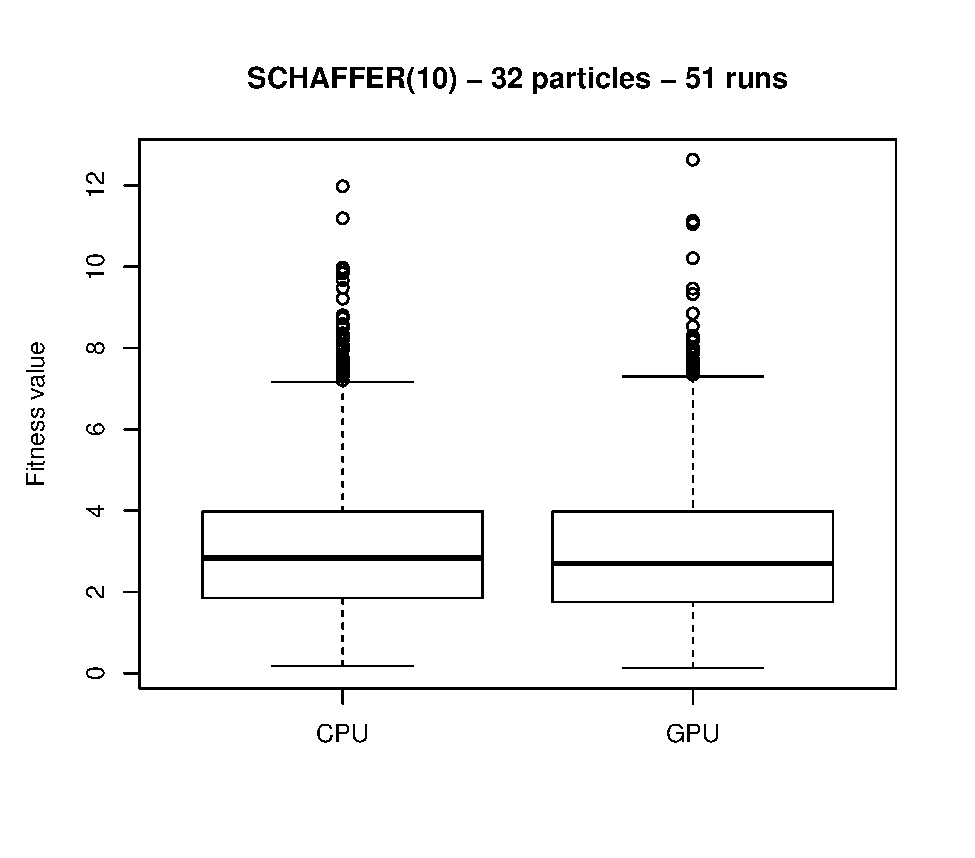
\includegraphics[width=.7\textwidth]{../img/schaffer10_32particles_fitness.eps}
        \caption{Boxplot of the quality of the solutions on the problem Schaffer with $10$ dimensions. In this experiment the GPU uses $51$ blocks of $32$ threads and the experiment was repeated $30$ times. The quality of the result is similar as they implement the same algorithm.}
        \label{fig:schaffer10_32particles_fitness}
    \end{figure}

    
    \begin{figure}[!htb]
        \centering
        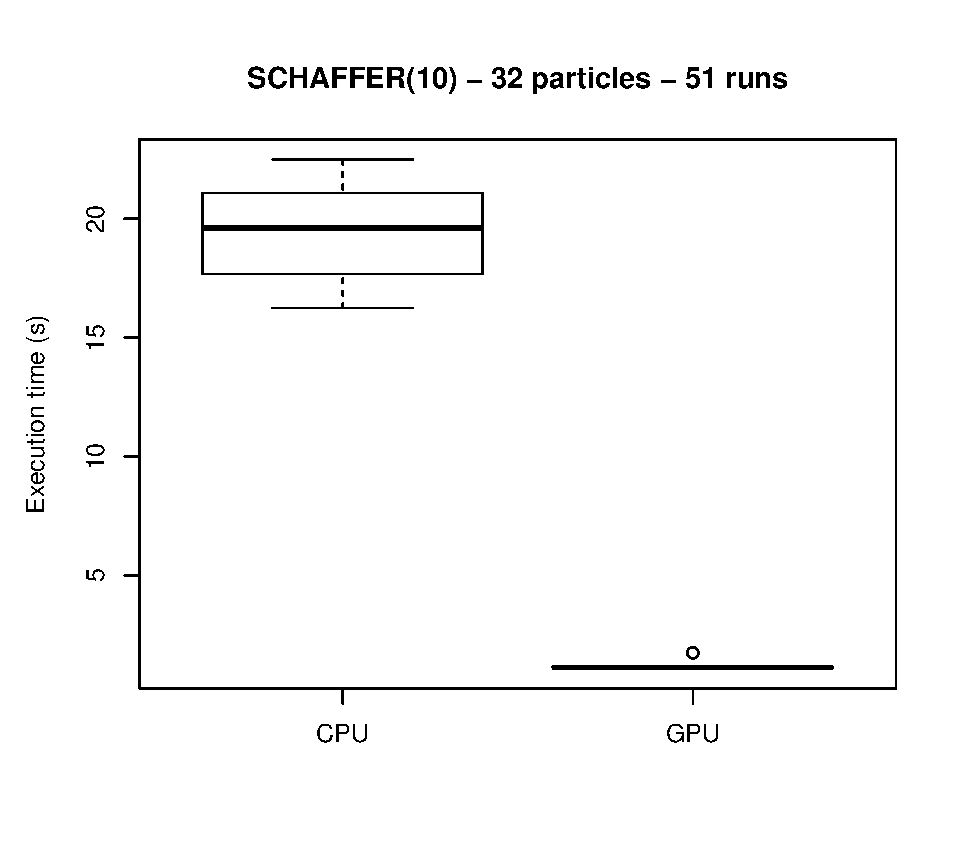
\includegraphics[width=.7\textwidth]{../img/schaffer10_32particles_time.eps}
        \caption{Boxplot of the execution time (in seconds) of GPU and CPU versions on the Shaffer problem with $10$ dimensions. In this experiment the GPU uses $51$ blocks of $32$ threads and the experiment was repeated $30$ times. The GPU version was about $16.8$ times faster then CPU.}
        \label{fig:schaffer10_32particles_time}
    \end{figure}

    To evaluate the scalability of the algorithms increasing the population size (and consequently the number of threads) an experiment was performed.
    The population size was set from $32$ up to $160$, increasing $32$ each time ({\it i.e.} \{$32$, $64$, $96$, $128$, $160$\}). The number of threads was not set above $160$ to exploit the use of shared memory. From Figure~\ref{fig:scalability_schafferf7} it is possible to observe that the quality of the solutions improve increasing the population size. Also, both CPU and GPU obtain equivalent results (in terms of quality of output) mainly from $32$ to $64$.

    \begin{figure}[!htb]
        \centering
        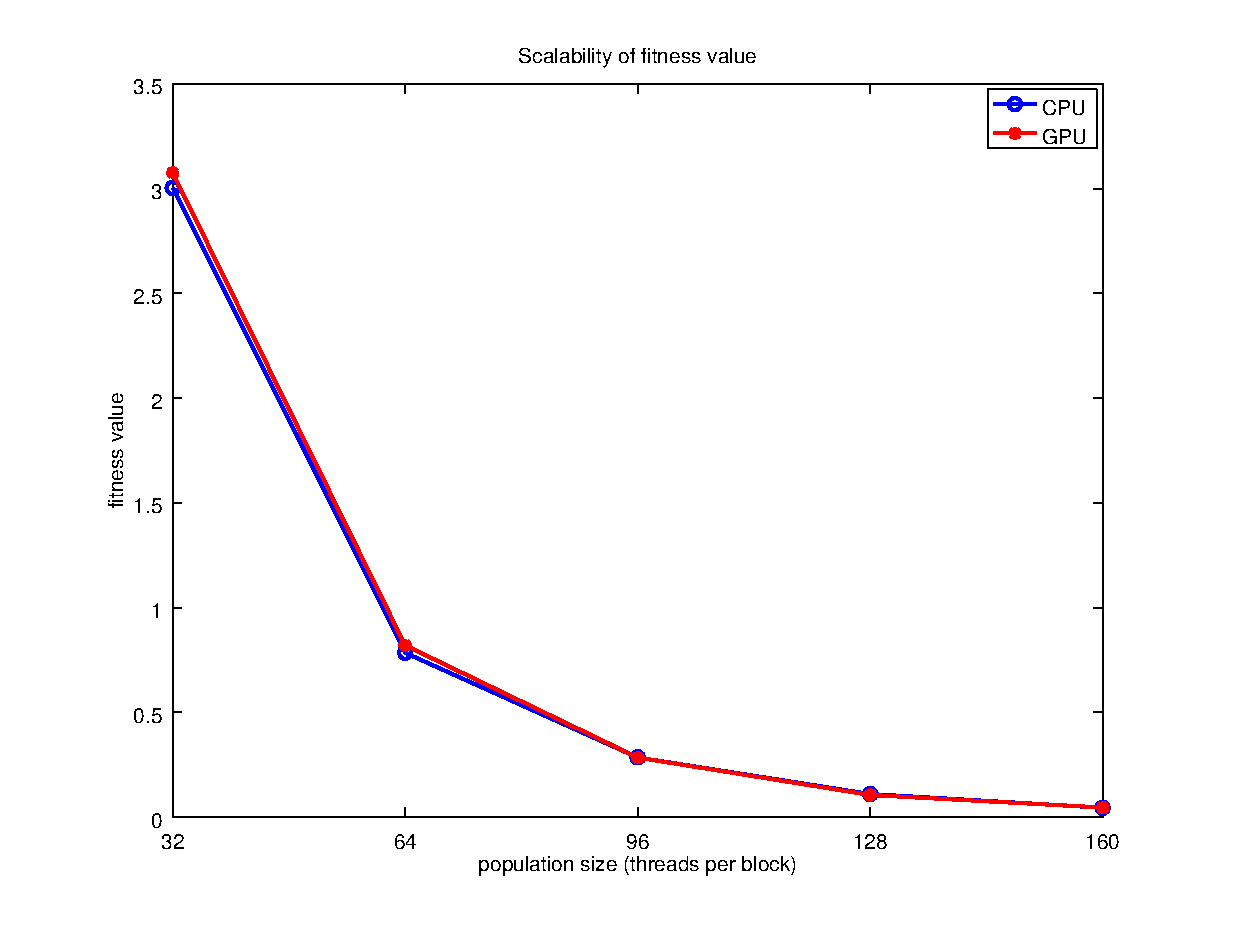
\includegraphics[width=.7\textwidth]{../img/scalability_schafferf7.eps}
        \caption{Scalability of the quality: average quality of the implementations (CPU and GPU) when increasing the population size. In this experiment the GPU uses $51$ blocks and the population size defines the number of threads. The experiment was repeated $30$ times. Both algorithms perform similarly, as much more population size, better the quality of the solutions.}
        \label{fig:scalability_schafferf7}
    \end{figure}

    It was also evaluated the scalability in terms of execution time (Figure~\ref{fig:scalability_schafferf7_time}).
    For both GPU and CPU increasing the population size (threads per block) increases the execution time.
    Although, the CPU time increases more drastically. From $32$ to $160$ the CPU execution time increased from $23.8$ seconds to $108.7$ seconds, while the GPU time increased from $1.22$ seconds to $5.45$. The Table~\ref{tbl:scalability} presents the scalability of GPU and CPU increasing the population size. 

 %% TODO descerever a tabela.


    \begin{figure}[!htb]
        \centering
        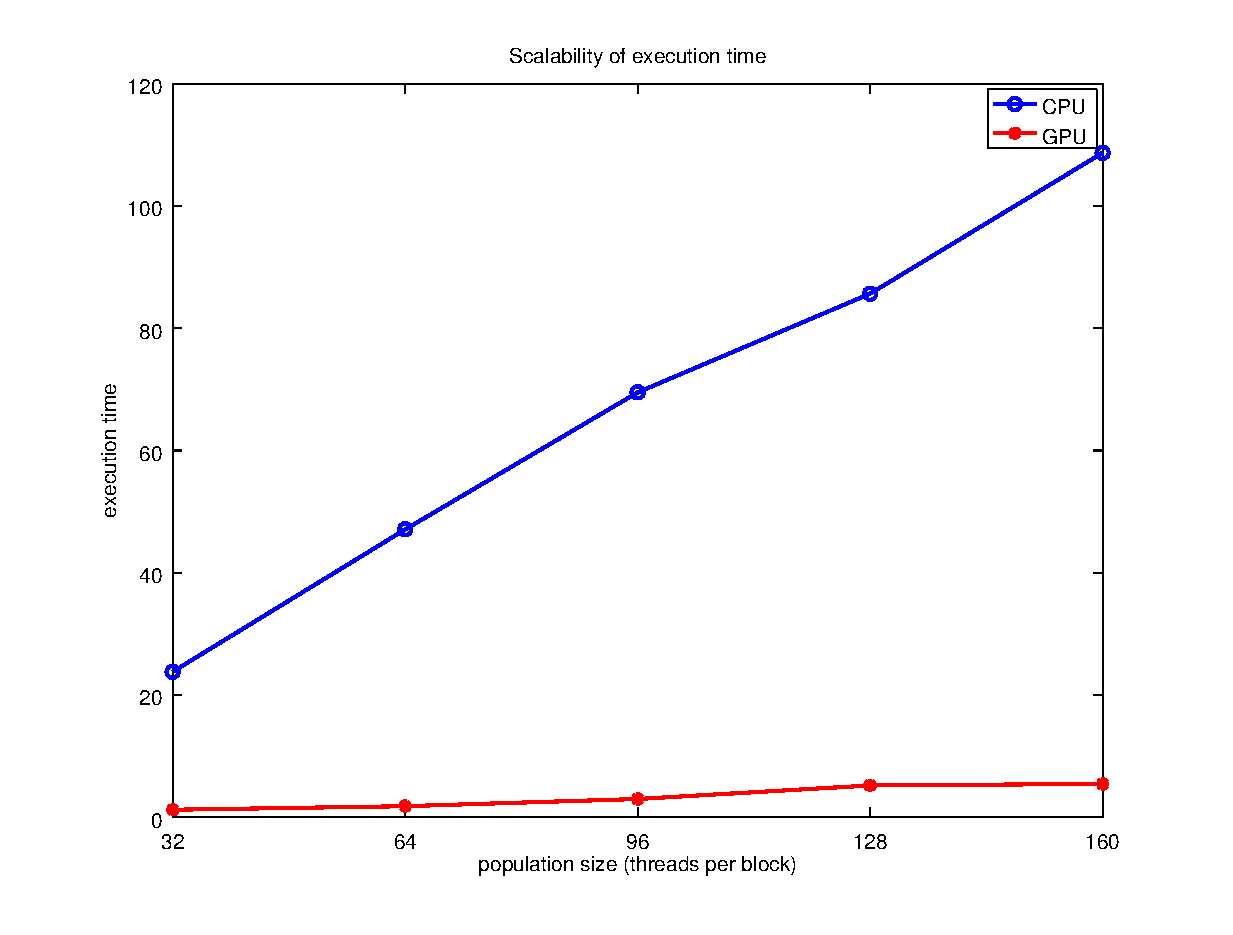
\includegraphics[width=.7\textwidth]{../img/scalability_schafferf7_time.eps}
        \caption{Scalability of the execution time (in seconds): average execution time (s) of the implementations (CPU and GPU) when increasing the population size. In this experiment the GPU uses $51$ blocks and the population size defines the number of threads. The experiment was repeated $30$ times. The average GPU speed up was $21$ times faster than CPU. From $32$ to $160$  threads the CPU execution time increased from $23.8$ seconds to $108.7$ seconds, while the GPU time increased from $1.22$ seconds to $5.45$.}
        \label{fig:scalability_schafferf7_time}
    \end{figure}

    \begin{table}[!htb]
        \centering
        \caption{Scalability of GPU and CPU increasing the population size. In this experiment the GPU uses $51$ blocks and the population size defines the number of threads. The experiment was repeated $30$ times. The best speed up was achived using $64$ threads per block while the worst was using $128$ threads per block.}
        \label{tbl:scalability}
        \begin{tabular}{|c|r|r|r|}
        \hline
        \textbf{population (threads)} & \multicolumn{1}{c|}{\textbf{GPU time (s)}} & \multicolumn{1}{c|}{\textbf{CPU time (s)}} & \multicolumn{1}{c|}{\textbf{GPU speed up}} \\ \hline
        32                       & 1.2274                                     & 23.8012                                    & 19.3909x                                   \\ \hline
        64                       & 1.8086                                     & 47.0796                                    & 26.0313x                                   \\ \hline
        96                       & 2.9866                                     & 69.5055                                    & 23.2725x                                   \\ \hline
        128                      & 5.2027                                     & 85.6585                                    & 16.4643x                                   \\ \hline
        160                      & 5.4543                                     & 108.7034                                   & 19.9297x                                   \\ \hline
        \end{tabular}
    \end{table}


    \section{Conclusions}

    In this project, we implement a Parallel Standard Particle Swarm Optimization.
    First, we compare the implementations regarding convergence quality, in which both GPU and CPU implementations were similar.
    After different implementations and experiments, it was possible to achieve a 12.054 speed up. The execution time of the CPU version for 51 runs was 12.84892 seconds (in an average of 30 repetitions). Moreover, the execution time for the GPU version was 1.065946 seconds.

    \bibliographystyle{plain}
    \bibliography{bibliography} 

\end{document}
